\newpage

\section*{Attachments}
% \begin{minipage}{0.8\textwidth}
\begin{figure}[h]
    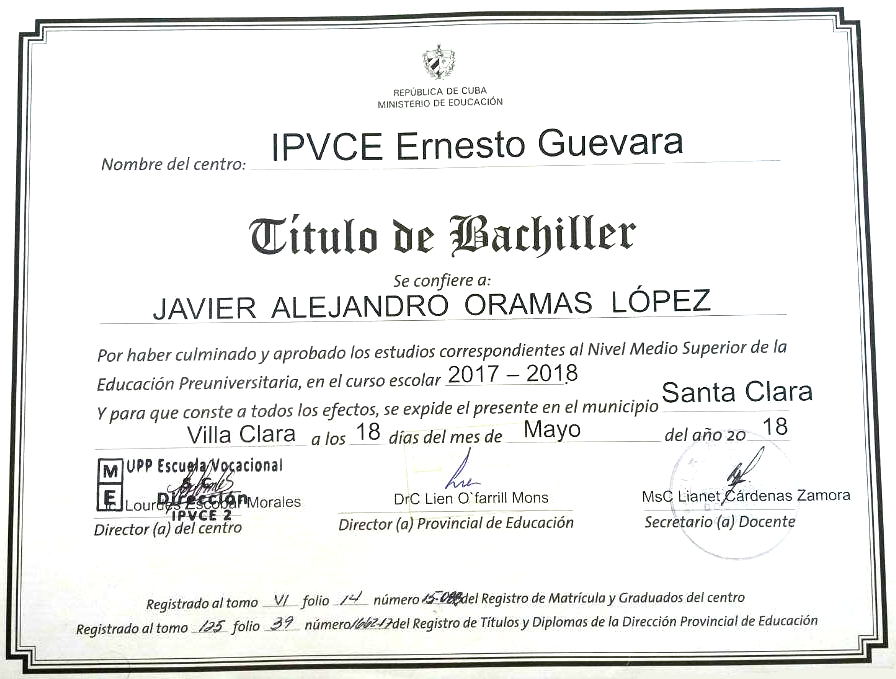
\includegraphics[width=\textwidth]{images/bachelor.png}
    \caption{Science Bachelor certificate}
    \label{sec:bachelor}
\end{figure}

\begin{figure}[h]
    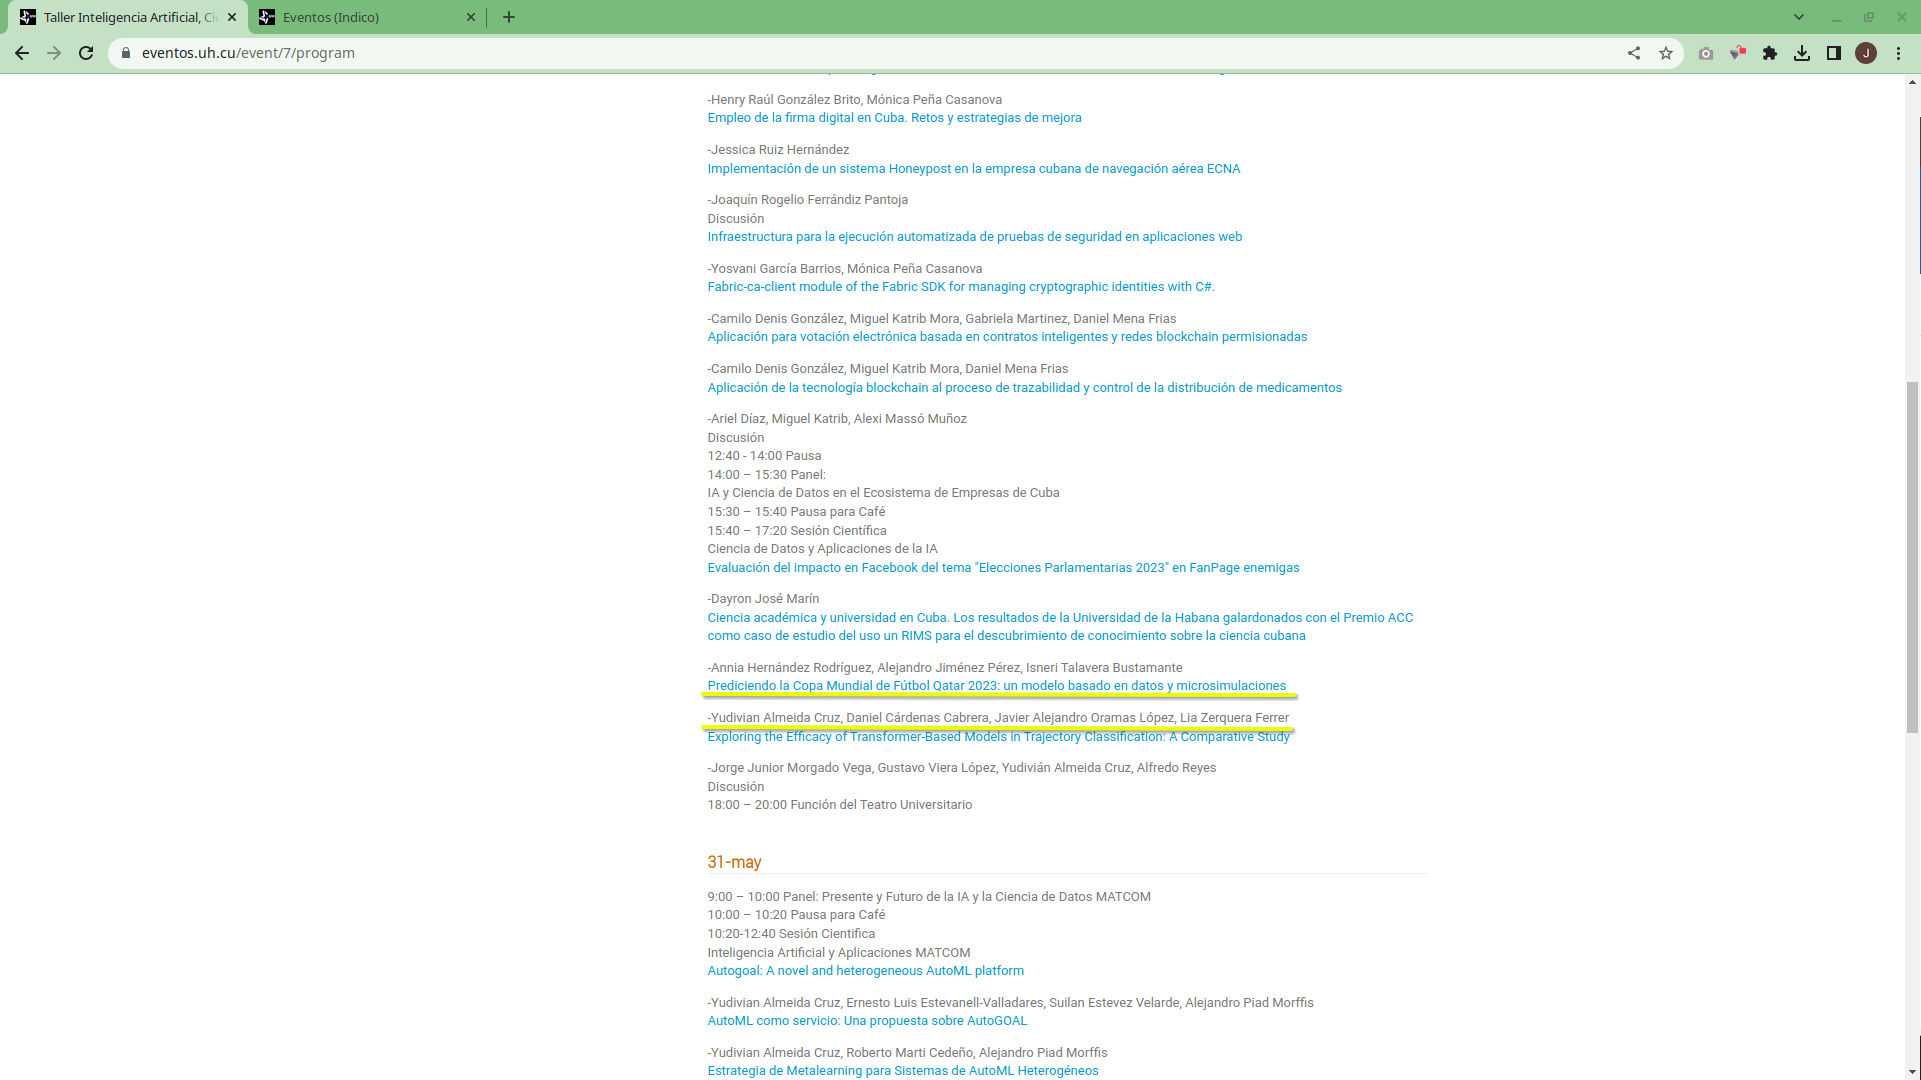
\includegraphics[width=\textwidth]{images/ai_workshop.png}
    \caption{\href{https://eventos.uh.cu/event/7/program}{Havana University events webpage}, screenshot 06/01/2023}
    \label{sec:workshop}
\end{figure}

\begin{figure}[h]
    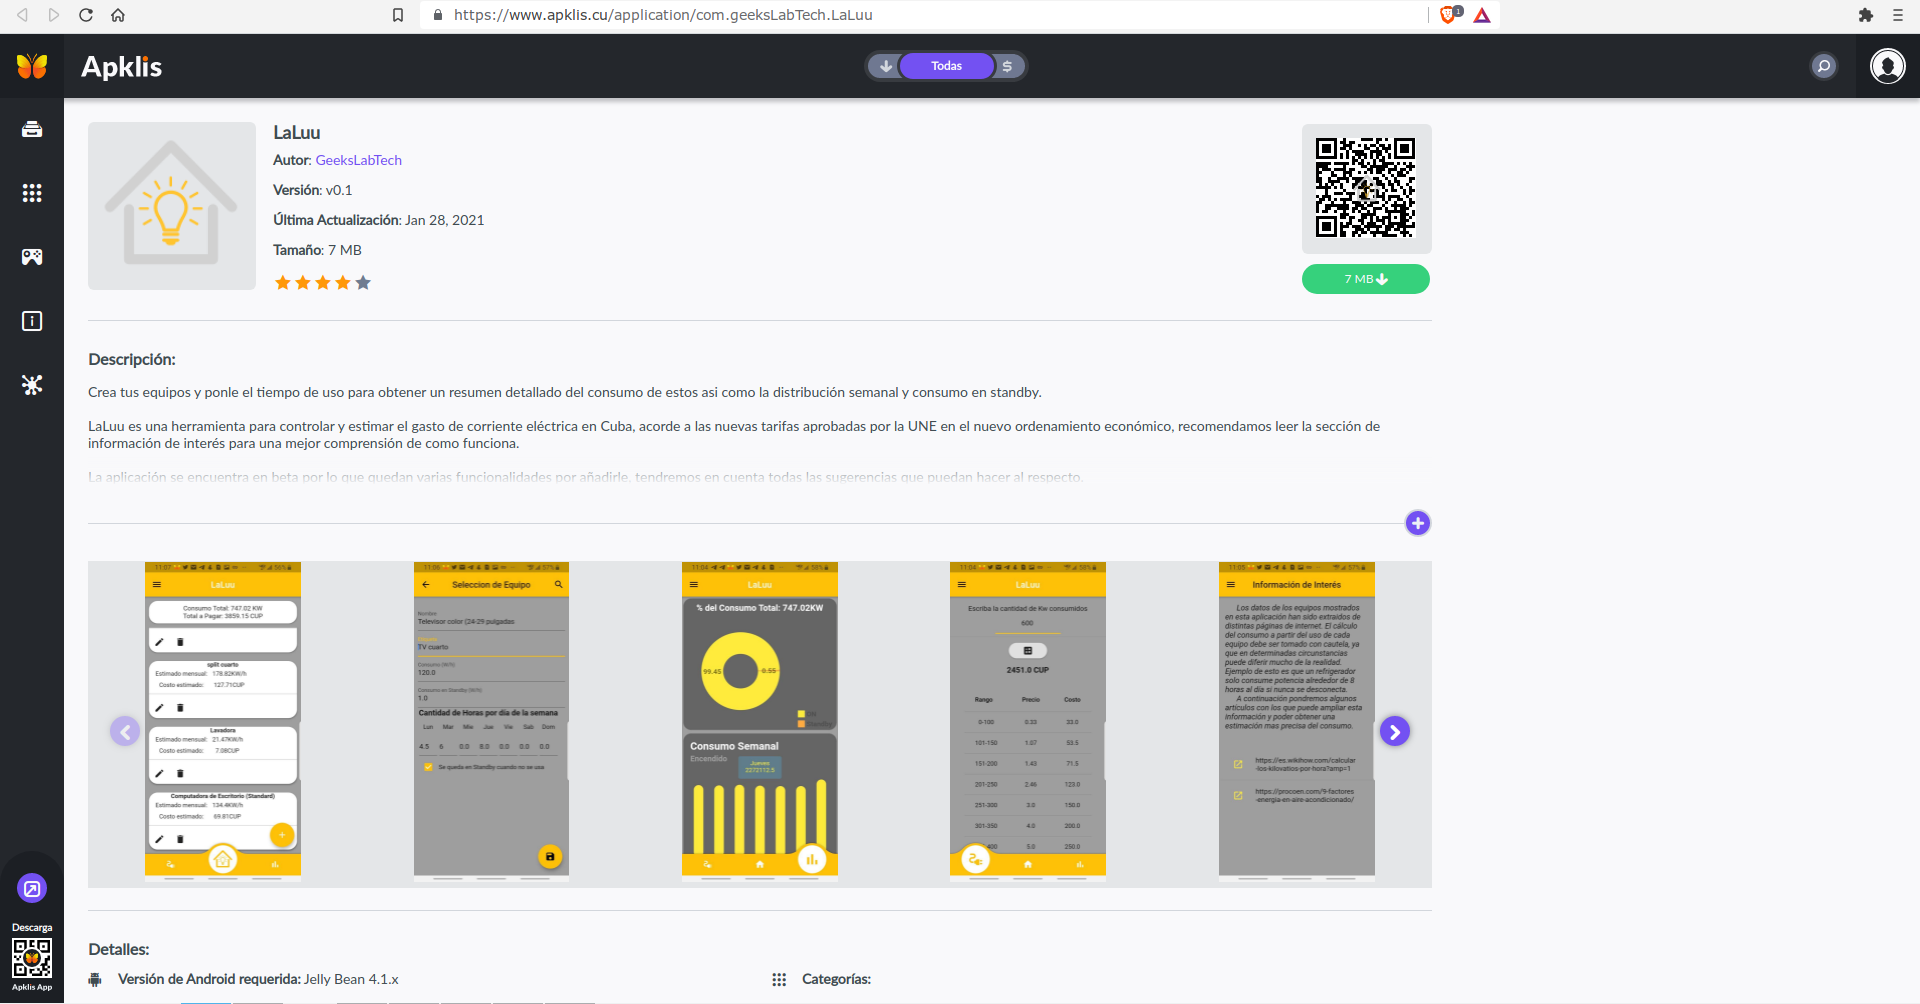
\includegraphics[width=\textwidth]{images/laluu.png}
    \caption{LaLuu app for estimation of Energy consumption. Available in \href{https://www.apklis.cu/application/com.geeksLabTech.LaLuu}{Apklis}, Cuban android app store, screenshot 01/25/2022}
    \label{sec:laluu}
\end{figure}

\begin{figure}[h]
    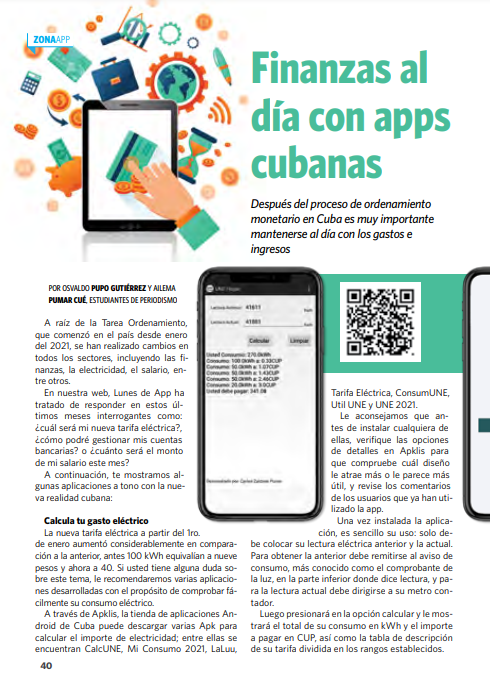
\includegraphics[width=\textwidth]{images/laluu_jt.png}
    \caption{Pupo, Gutiérrez O. y Pumar, Cué A. (may-jun 2021). \href{http://www.juventudtecnica.cu/sites/default/files/jt_420.pdf}{Finanzas al día con apps cubanas}. Juventud Técnica 420 (40-41), ISSN: 0449-4555, screenshot 01/25/2022}
    \label{sec:laluu_press}
\end{figure}

\begin{figure}[h]
    
\includegraphics[width=\textwidth]{images/laluu_art.png}
    \caption{Red Artemisa (february 2nd 2021).\href{https://www.artemisa.gob.cu/es/actualidad/noticias/9806-llego-febrero-calcula-tu-gasto-electrico-con-esta-apps}{Llegó febrero: calcula tu gasto eléctrico con esta apps.}, screenshot 01/25/2022}
\end{figure}

\begin{figure}[h]
    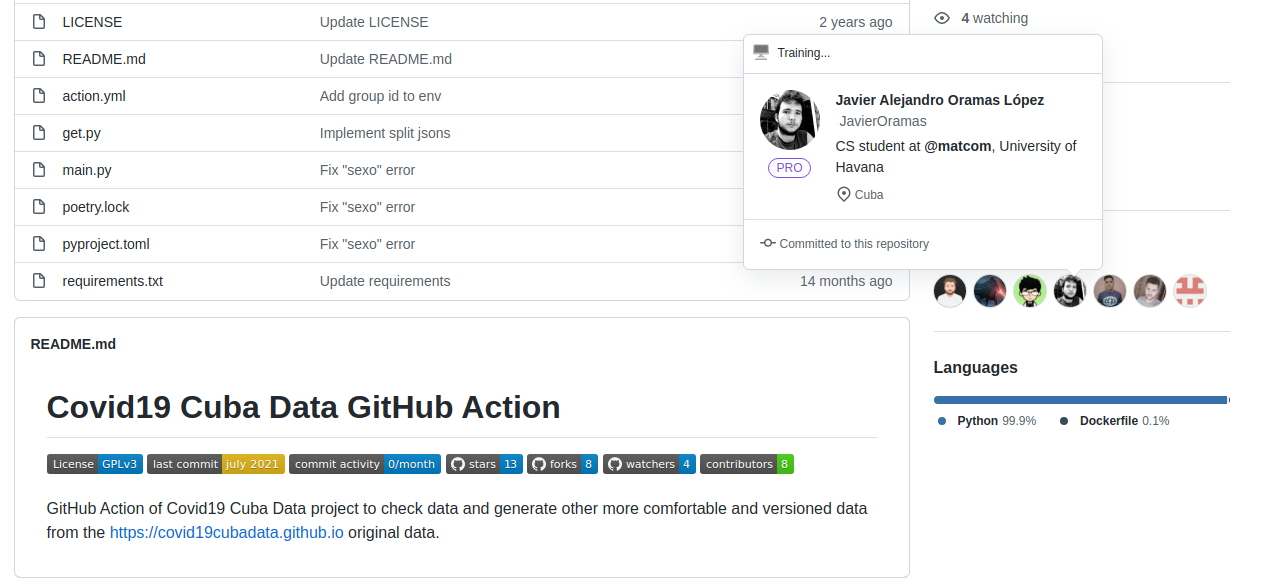
\includegraphics[width=\textwidth]{images/covid_19.png}
    \caption{\href{https://github.com/covid19cuba/covid19cuba-action}{Covid19CubaData app COVID-19 data analisys in Cuba}, screenshot 01/25/2022}
    \label{sec:covid}
\end{figure}

\begin{figure}[h]
    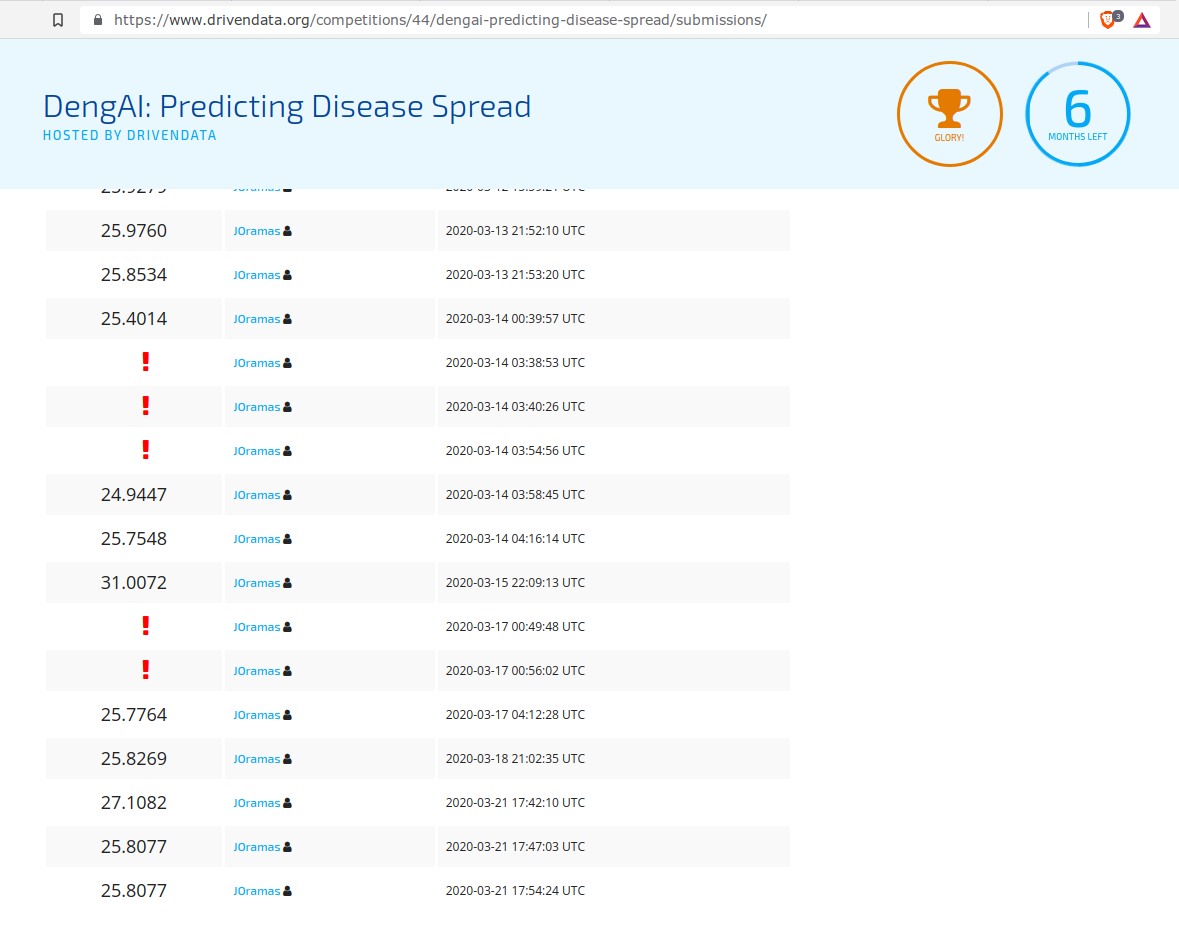
\includegraphics[width=\textwidth]{images/dengue.png}
    \caption{Competition Predicting Dengue Cases based on metheorological variables, using Machine Learning and Deep Learning. \href{https://www.drivendata.org/competitions/44/dengai-predicting-disease-spread}{DrivenData}, screenshot 01/25/2022}
    \label{sec:dengue}
\end{figure}

\begin{figure}[h]
    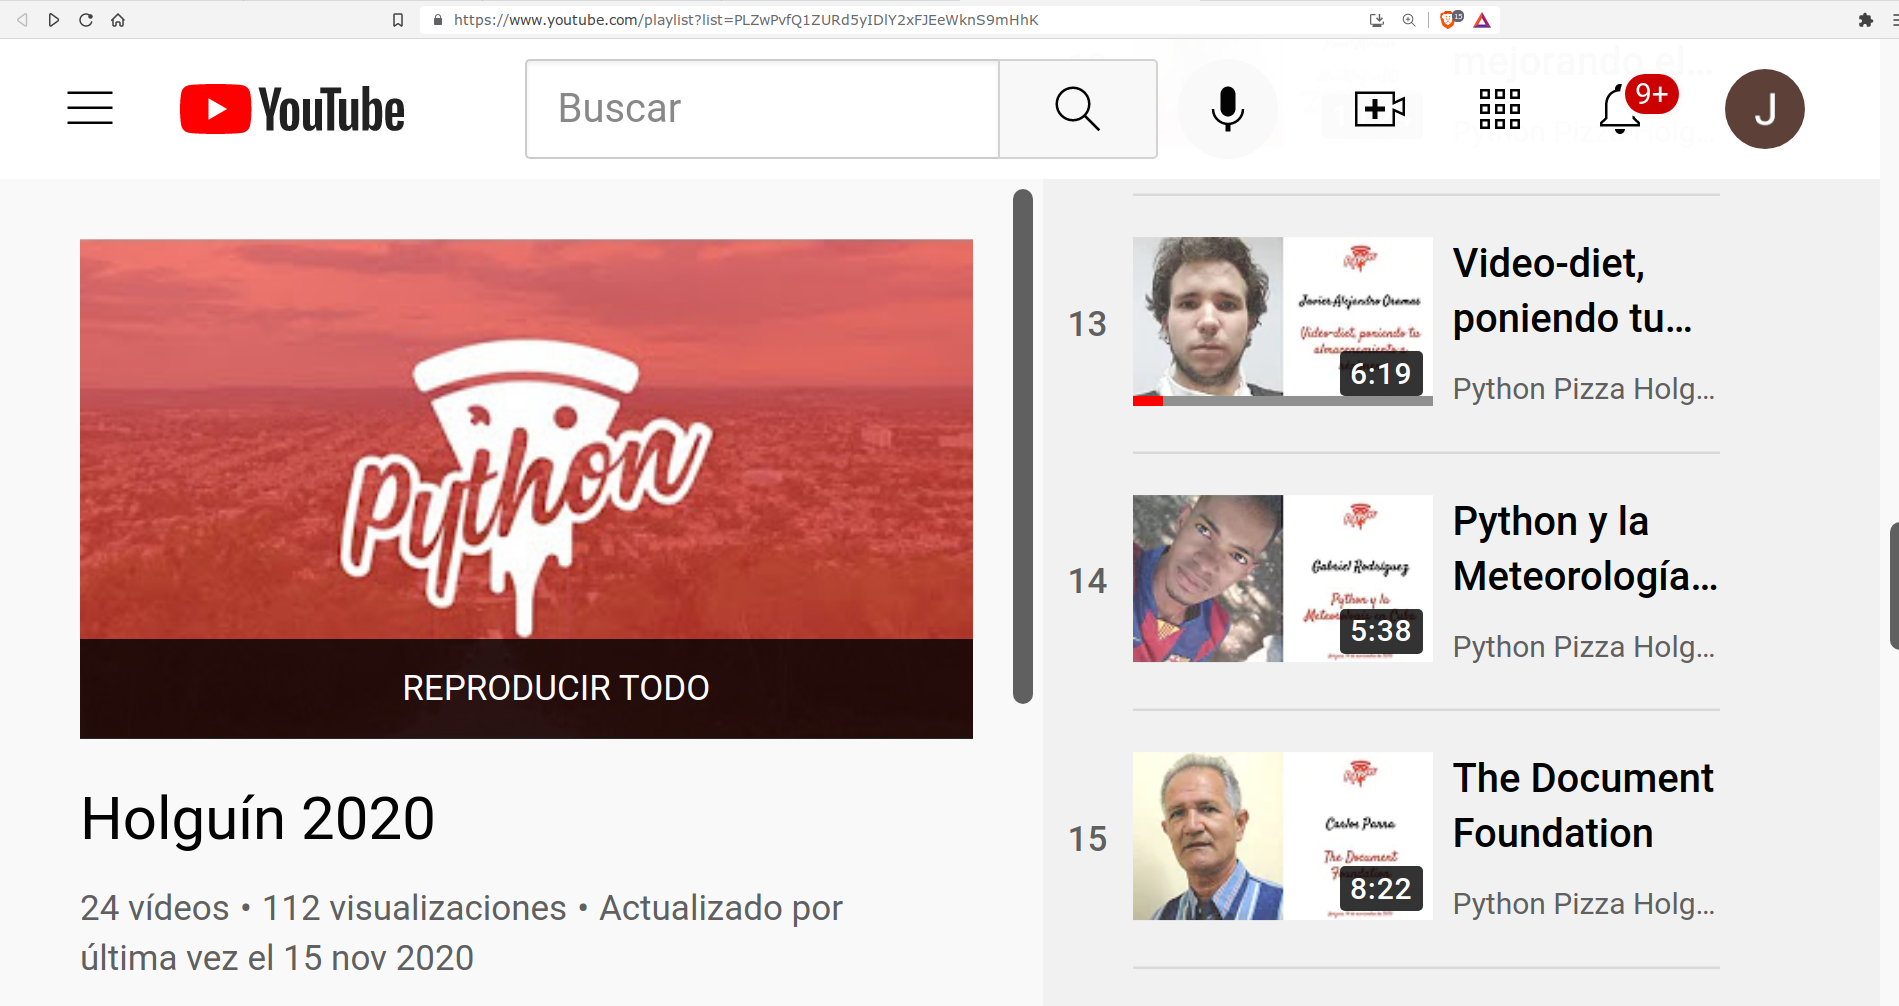
\includegraphics[width=\textwidth]{images/pythonpizza.png}
    \caption{Oramas, J. \href{https://holguin.python.pizza/?ref=python.pizza}{[Python Pizza Holguín]}. (nov 15th 2020). Video-Diet: poniendo a dieta tu almacenamiento \href{https://youtu.be/c--NOwM5W-0}{[Video]}.screenshot 01/25/2022}
    \label{sec:pythonpizza}
\end{figure}

\begin{figure}[h]
    \centering
    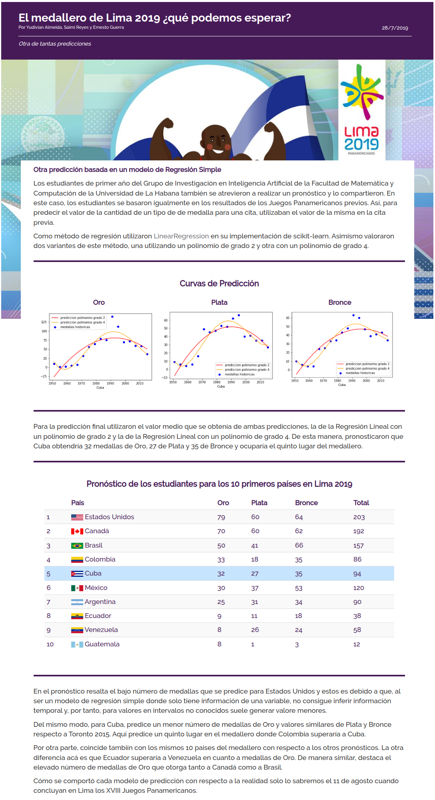
\includegraphics[height=0.8\textheight]{images/panamerican.png}
    \caption{\href{http://www.postdata.club/issues/201907/el-medallero-de-lima-2019-que-se-puede-esperar.html}{Almeida, Y. , Reyes, S. y Guerra, E. (jul 28th 2019). El medallero de Lima 2019 ¿qué podemos esperar? PostData.club Periodismo de Datos.}, screenshot 01/25/2022}
    \label{sec:panamerican}
\end{figure}

\begin{figure}[h]
    \centering
    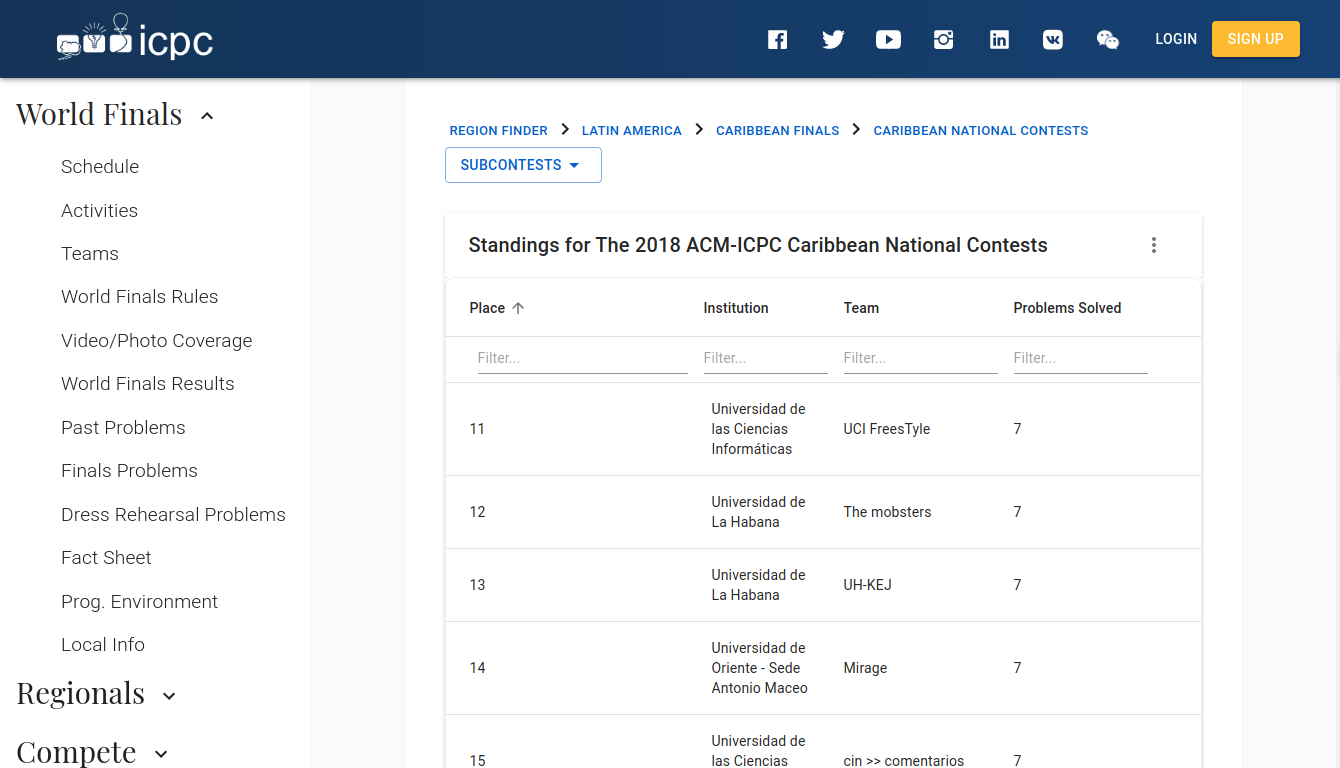
\includegraphics[width=\textwidth]{images/icpckej.png}
    \caption{ \href{https://icpc.global/regionals/finder/cnc-2018/standings}{International Collegiate Programming Contest (oct 2018). Standings for The 2018 ACM-ICPC Caribbean National Contests}. screenshot 01/25/2022}
    \label{sec:icpc_kej}
\end{figure}

\begin{figure}[h]
    \centering
    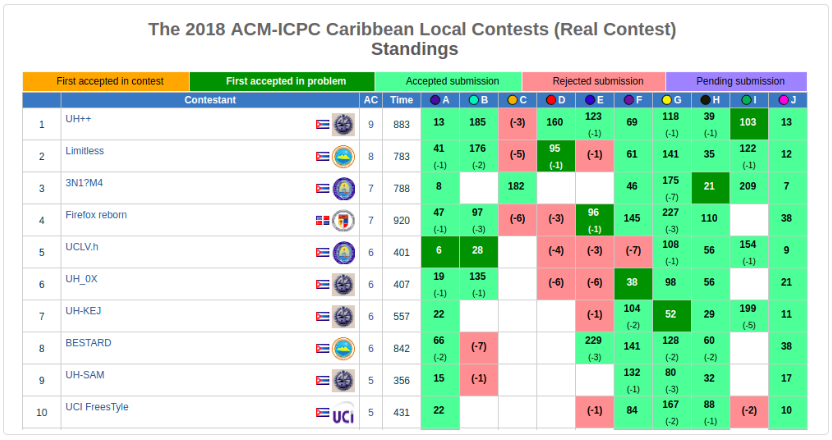
\includegraphics[width=\textwidth]{images/icpckej_standing.png}
    \caption{\href{https://matcomgrader.com/post/5179/resultados-del-concurso-local-caribeno-2018}{Matcom Online Grader (sept 2018). Resultados del Concurso Local Caribeño 2018. Facultad de Matemática y Ciencia de la Computación, Universidad de La Habana.}, screenshot 01/25/2022}
    % \label{sec:}
\end{figure}

\begin{figure}[h]
    \centering
    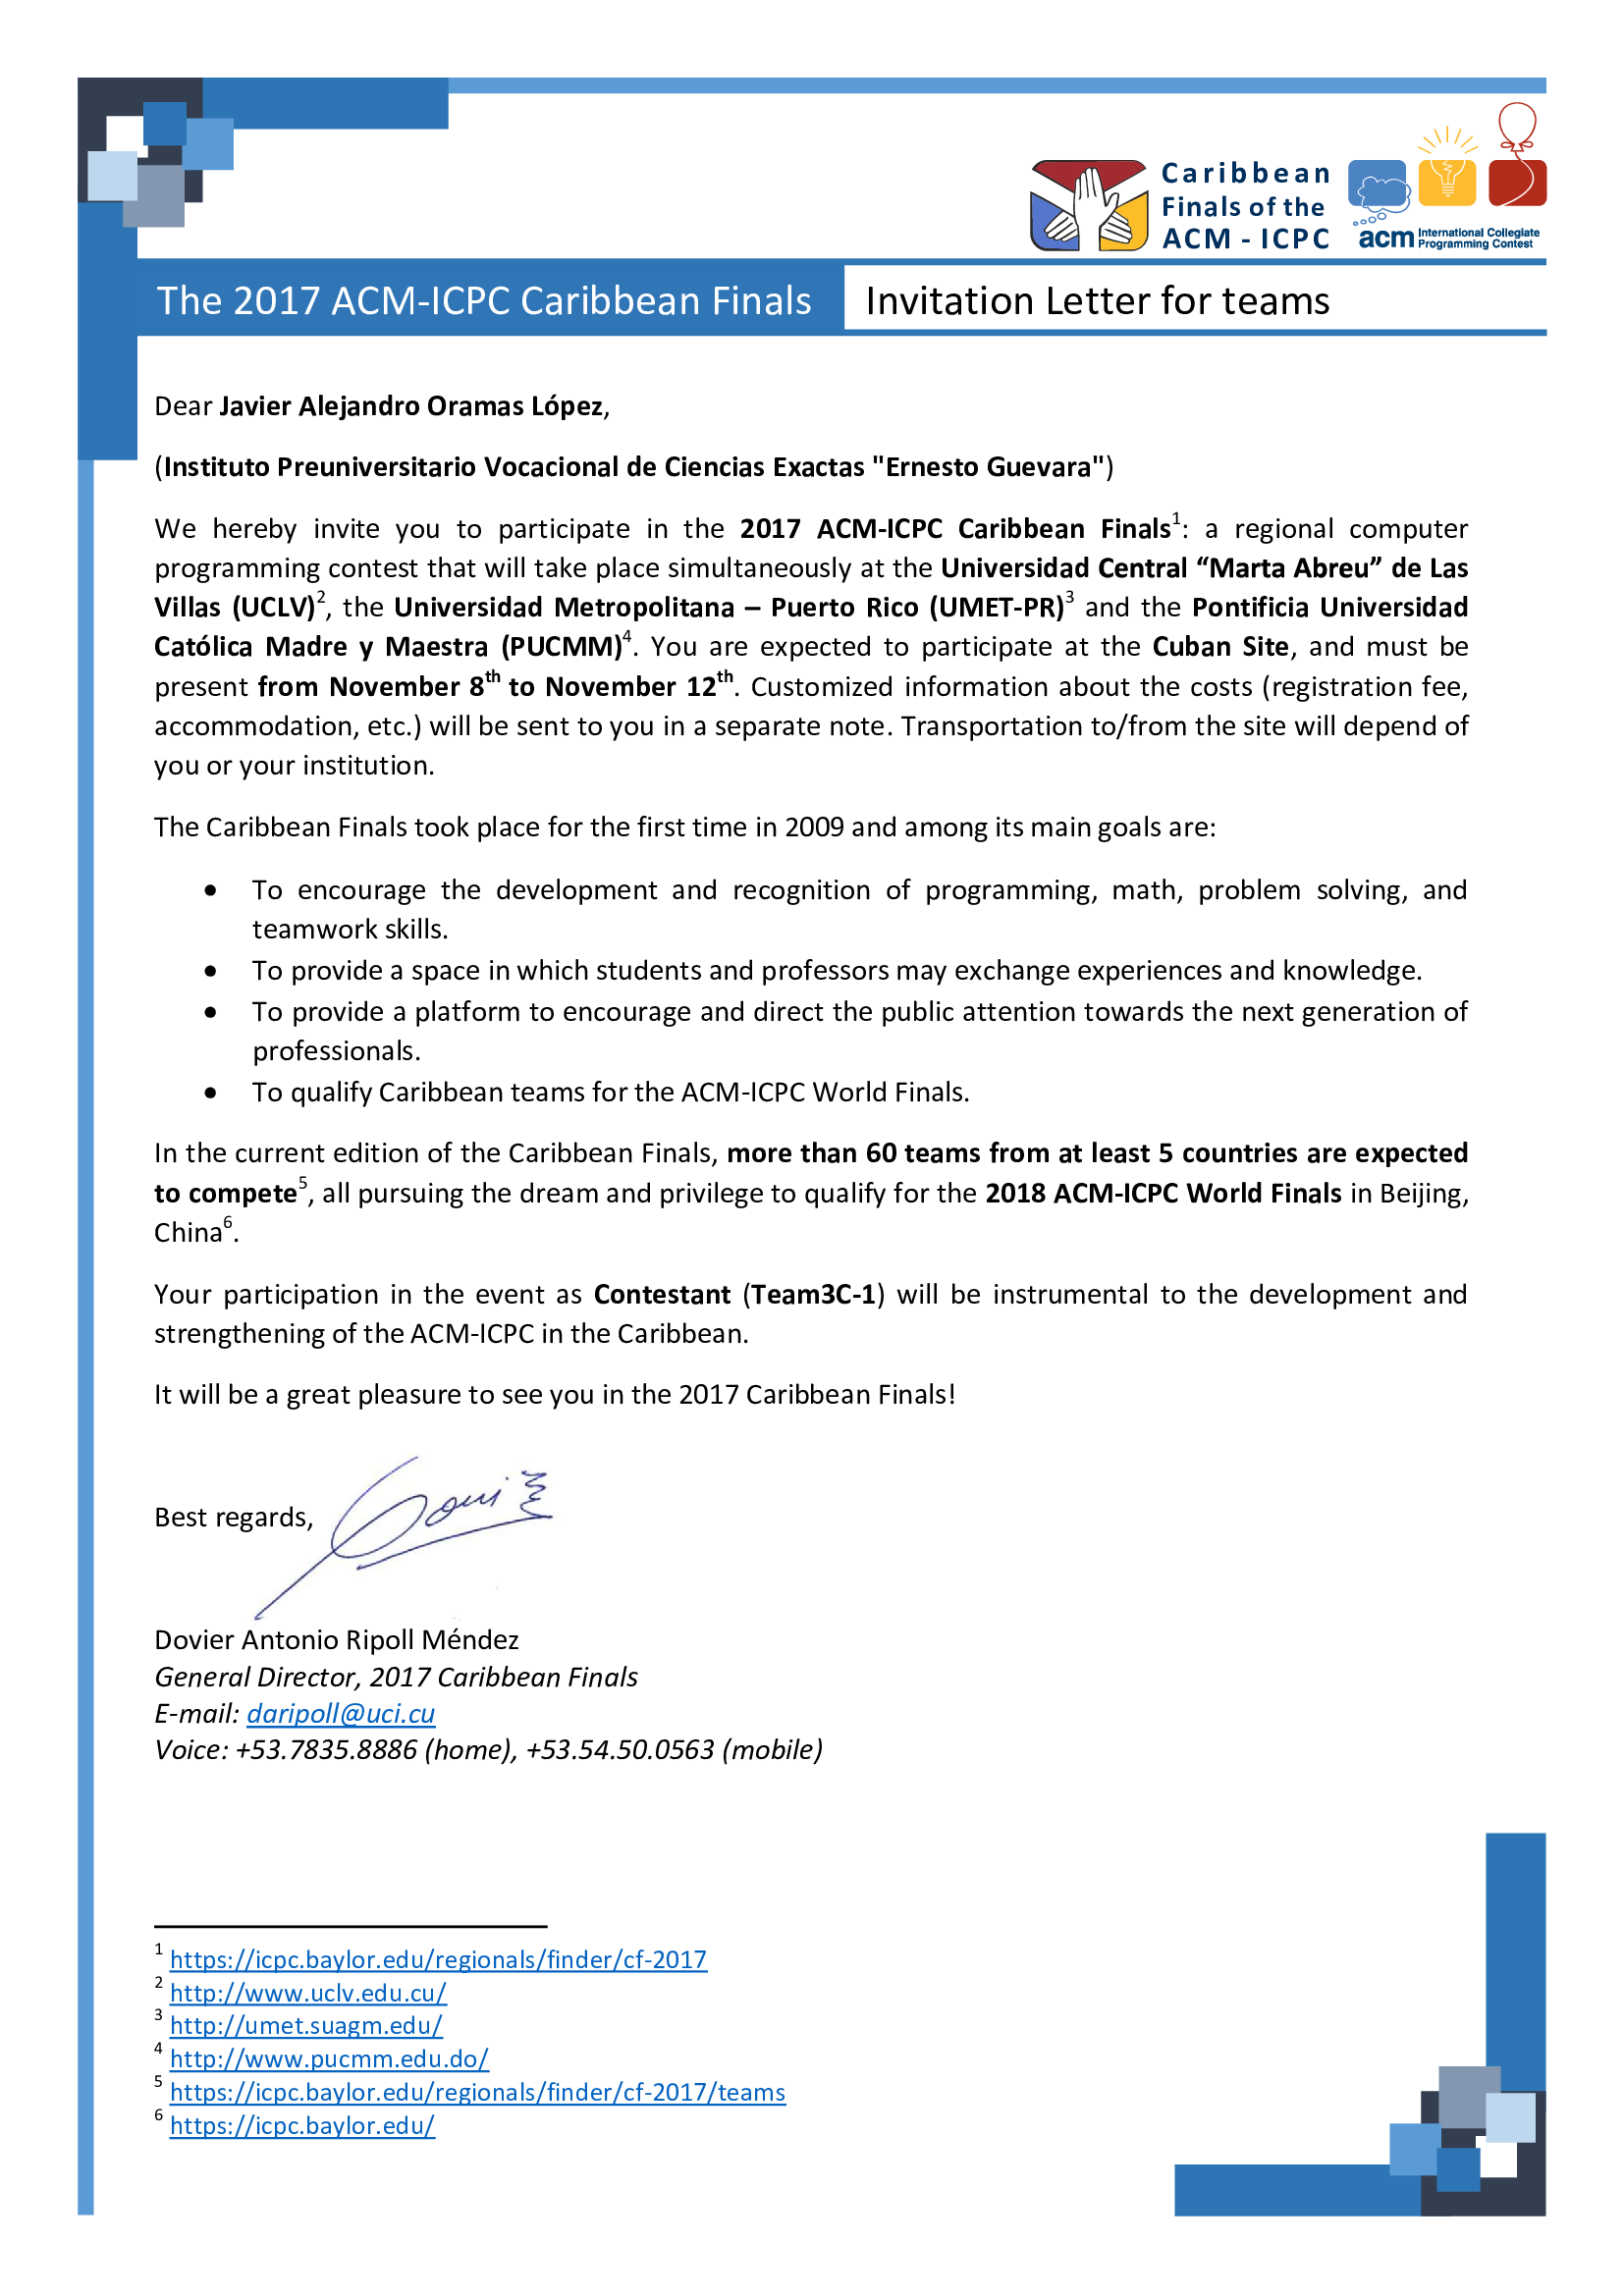
\includegraphics[width=\textwidth]{images/letter.png}
    \caption{General Director invitation letter, Caribbean Finals ACM - ICPC 2017, screenshot 01/25/2022}
    \label{sec:letter}
\end{figure}

\begin{figure}[h]
    \centering
    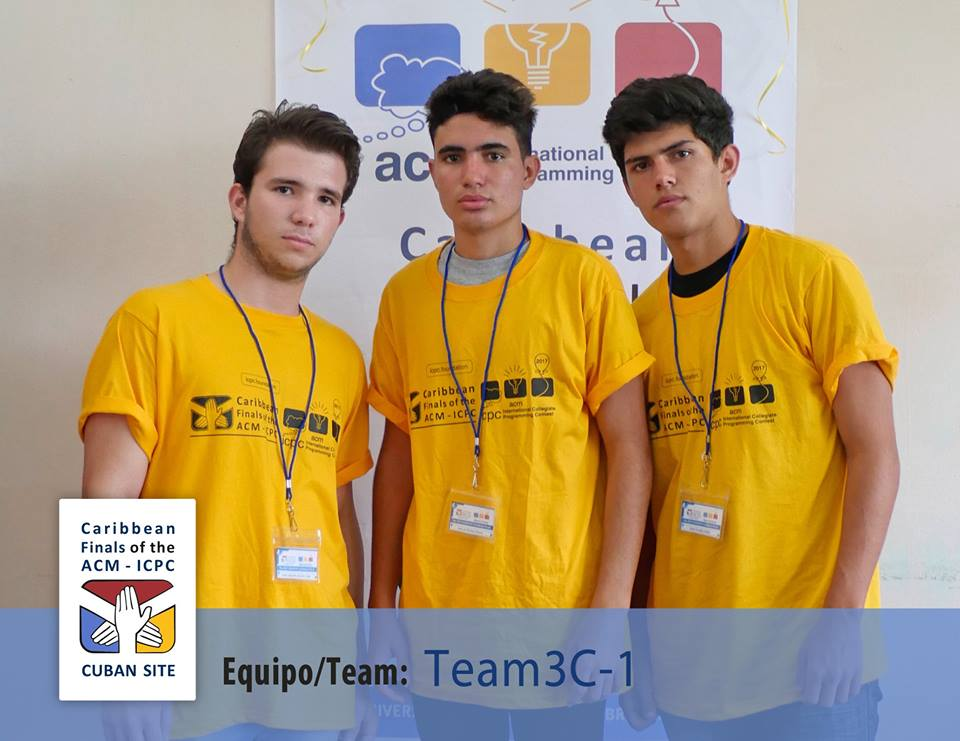
\includegraphics[width=\textwidth]{images/team3c.jpg}
    \caption{\href{https://matcomgrader.com/post/5167/the-2017-acm-icpc-caribbean-finals}{Matcom Online Grader (oct 2017). The 2017 ACM-ICPC Caribbean Finals. Facultad de Matem?tica y Ciencia de la Computaci?n, Universidad de La Habana} screenshot 01/25/2022}
    \label{sec:3c}
\end{figure}
\begin{figure}[h]
    \centering
    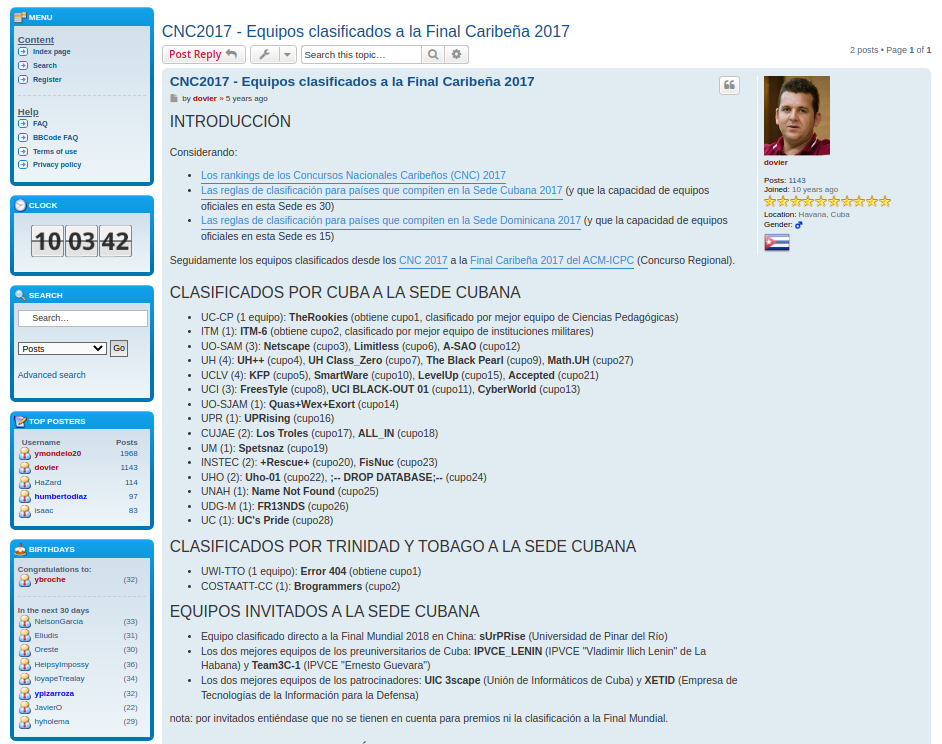
\includegraphics[width=\textwidth]{images/icpc_classified.png}
    \caption{\href{ https://coj-forum.uci.cu/viewtopic.php?t=3315}{Caribbean Online Judge (nov 2017). Final Caribe?a del ACM - ICPC 2017.}, screenshot 01/25/2022}
    \label{sec:icpc}
\end{figure}

\begin{figure}[h]
    \centering
    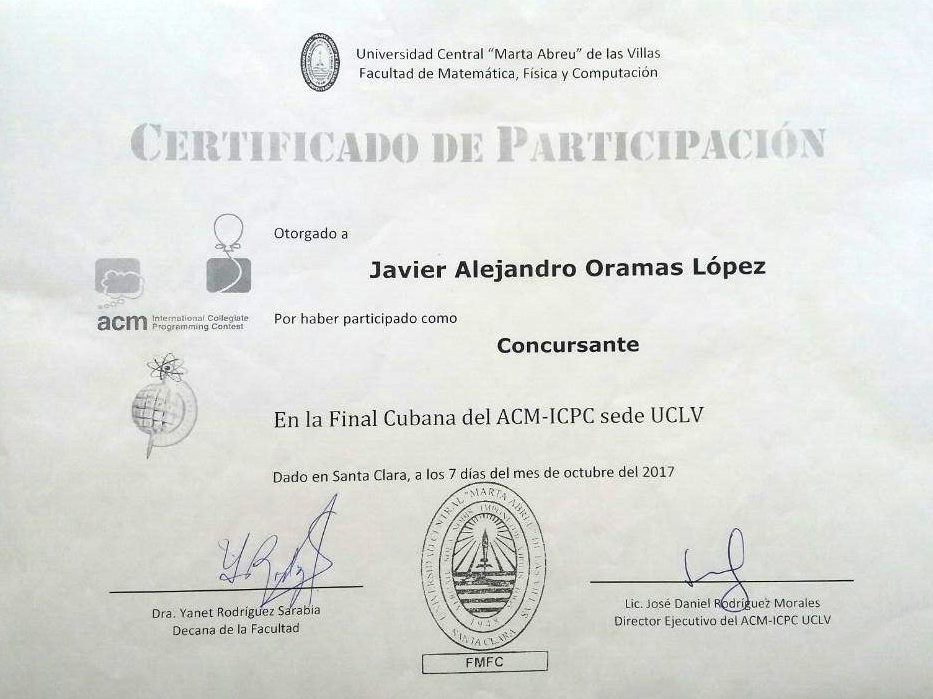
\includegraphics[width=\textwidth]{images/2017final.png}
    \caption{Participation Certificate, ACM-ICPC 2017 Cuban Finals, screenshot 01/25/2022}
    \label{sec:2017final}
\end{figure}


\begin{figure}[h]
    \centering
    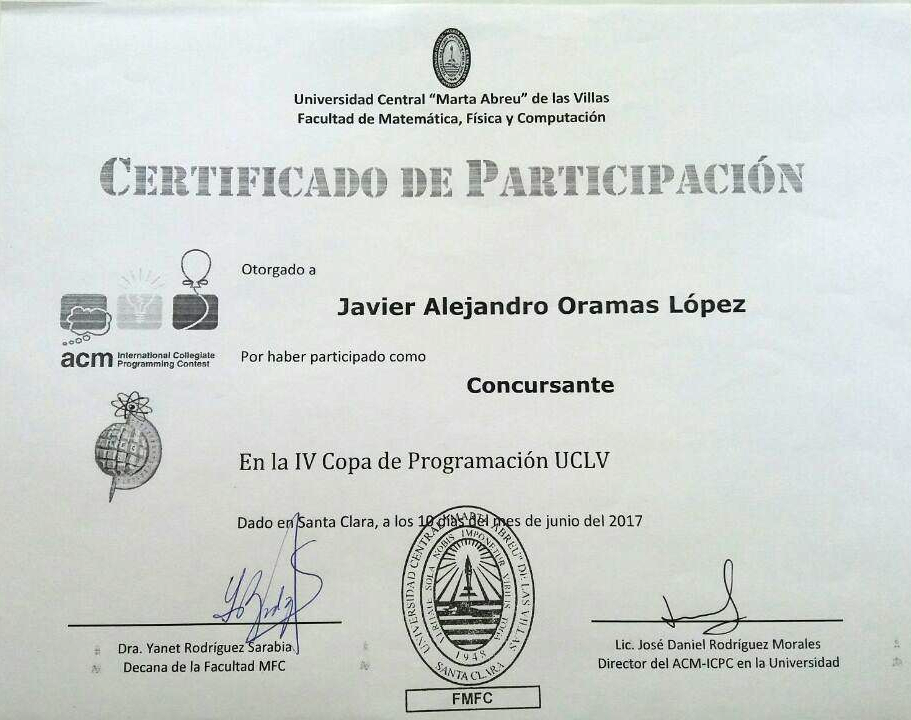
\includegraphics[width=\textwidth]{images/uclv_cup.png}
    \caption{Participation Certificate, IV Programming Cup, Universidad Central de Las Villas, screenshot 01/25/2022}
    \label{sec:uclv_cup}
\end{figure}


\begin{figure}[h]
    \centering
    
\includegraphics[width=\textwidth]{images/nac_contest.png}
    \caption{Certificate for Relevant Results obtained in the National Informatics Competition, Mach 2017, screenshot 01/25/2022}
    \label{sec:nac_contest}
\end{figure}


\begin{figure}[h]
    \centering
    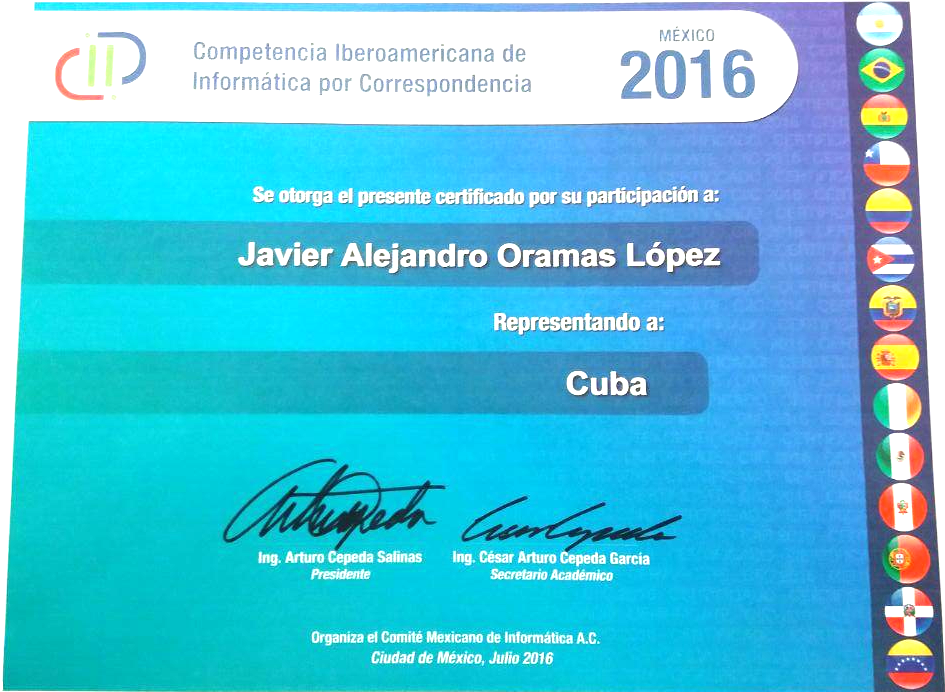
\includegraphics[width=\textwidth]{images/ibero.png}
    \caption{Certificate of Participation, Iberoamerican Computer Correspondence Competition, México 2016, screenshot 01/25/2022}
    \label{sec:ibero}
\end{figure}


\begin{figure}[h]
    \centering
    
\includegraphics[width=\textwidth]{images/preseleccion.png}
    \caption{Certificate from the Ministry of Education of Cuba for having integrated the National Preselection to the International Olympiads of Informatics. 2016, screenshot 01/25/2022}
    \label{sec:preseleccion}
\end{figure}


\begin{figure}[h]
    \centering
    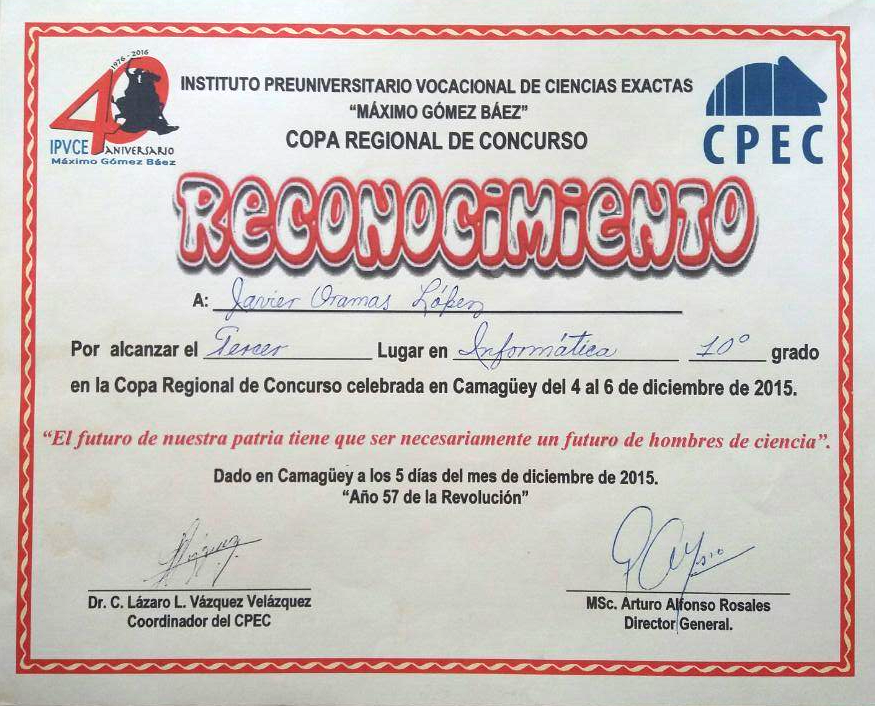
\includegraphics[width=\textwidth]{images/tinajon.png}
    \caption{Certificate for Third place obtained in the Regional Cup of Computer Science Competition, Camag\"uey December 2015, screenshot 01/25/2022}
    \label{sec:tinajon}
\end{figure}


\begin{figure}[h]
    \centering
    
\includegraphics[width=\textwidth]{images/2016nacional.png}
    \caption{Certificate of participation in the National Competition of the ACM-ICPC, Universidad Central de Las Villas, October 2015, screenshot 01/25/2022}
    \label{sec:nacional2016}
\end{figure}


\begin{figure}[h]
    \centering
    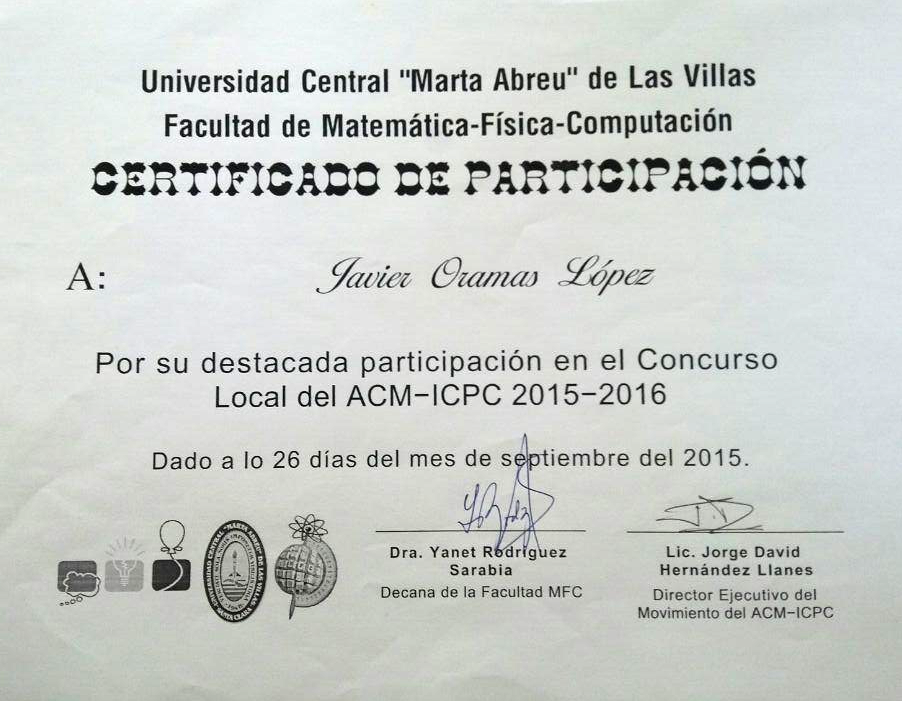
\includegraphics[width=\textwidth]{images/2016local.png}
    \caption{Certificate of participation in the Local Competition of the ACM-ICPC, Universidad Central de Las Villas, September 2015, screenshot 01/25/2022}
    \label{sec:local2016}
\end{figure}

\begin{figure}[h]
    \centering
    
\includegraphics[width=\textwidth]{images/informatica.png}
    \caption{Recognition for second place obtained in the National Computer Science Competition, Marzo 2014, screenshot 01/25/2022}
    \label{sec:informatic}
\end{figure}
